\documentclass{beamer}

\usepackage{amsmath}
\usepackage{amssymb}

\begin{document}
	%======================================================= % 
	%	\item Measuring risk in a micro dataset is a key task. Risk measurements are essential
	%	to determine if the dataset is secure enough to be released. To assess disclosure
	%	risk, one must make realistic assumptions about the information data users might
	%	have at hand to match against the micro dataset, these assumptions are called
	%	disclosure risk scenarios. 
	%	
	%	\item This goes hand in hand with the selection of categorical
	%	key variables because the choice these identifying variables defines a specific dis-
	%	closure risk scenario. 
	%	\item The specific set of chosen key variables has direct influence
	%	on the risk assessment because their distribution is a key input for the calculation
	%	of both individual and global risk measures as it is now discussed.
	%------------------------------------------------------------------------------%
\begin{frame}	
\frametitle{Measuring Risk}
\begin{itemize}
\item Measuring risk in a micro dataset is a key task. Risk measurements are essential
	to determine if the dataset is secure enough to be released. 
\item To assess disclosure
	risk, one must make realistic assumptions about the information data users might
	have at hand to match against the micro dataset; these assumptions are called
	disclosure risk scenarios. 
\item This goes hand in hand with the selection of categorical
	key variables because the choice these identifying variables defines a specific disclosure risk scenario. 
\end{itemize}
\end{frame}
%\begin{frame}	
%	\frametitle{Measuring Risk}
%	\begin{itemize}
%		\item The specific set of chosen key variables has direct influence on
%	the risk assessment because their distribution is a key input for the estimation of
%	both individual and global risk measures as it is now discussed. \item For example, for a
%	disclosure scenario for the European Union Structure of Earnings Statistics we can
%	assume that information on company size, economic activity, age and earnings of
%	employees are available in available data bases. \item Based on a specific disclosure risk
%	scenario, it is necessary to define a set of key variables (i.e., identifying variables)
%	that can be used as input for the risk evaluation procedure.
%	% Usually different scenarios are considered. 
%\end{itemize}
%\end{frame}
%\begin{frame}	
%	\frametitle{Measuring Risk}
%	\begin{itemize}
%	
%	\item For example, for the European Union Structure of Earnings
%	Statistics a second scenario based on an additional key varibles is of interest to
%	look at. e.g. occupation might be considered  well as an categorical key variable.
%	\item The resulting risk might now be higher than for the previous scenario. It needs
%	discussion with subject matter specialists which scenario is most realistic and an
%	evaluation of different scenarios helps to get a broader picture about the disclosure
%	risk in the data.
%\end{itemize}
%\end{frame}
%---------------------------------------------------------------------------------%
\subsection*{Population Frequencies and the Individual Risk Appoach}
\begin{frame}	
	\frametitle{Population Frequencies}
	\begin{itemize}
		\item 
	\item Typically, risk evaluation is based on the concept of uniqueness in the sample
	and / or in the population. The focus is on individual units that possess rare com	binations of selected key variables.
	\item The assumption is that units having rare
	combinations of key variables can be more easily identified and thus have a higher
	risk of re-identification/disclosure. 
	\item It is possible to cross-tabulate all identifying
	variables and view their cast. 
	\item Keys possessed by only very few individuals are
	considered risky, especially if these observations also have small sampling weights.
	This means that the expected number of individuals with these patterns is expected to be low in the population as well.
\end{itemize}
\end{frame}
%% -- Page 6 / 31
%% 2 MEASURING THE DISCLOSURE RISK
\begin{frame}	
	\frametitle{Population Frequencies}

\begin{itemize}
	\item To assess whether a unit is at risk, a threshold approach is typically used. If the
	risk of re—identification for an individual is above a certain threshold value, the unit
	is said to be at risk. 
	\item To compute individual risks, it is necessary to estimate the
	frequency of a given key pattern in the population. 
	
	\item Let us define frequency counts
	in a mathematical notation. Consider a random sample of size n drawn from a
	finite population of size N. Let $\pi_j$, $j = 1, \ldots ,N$ be the (first order) inclusion
	probabilities — the probability that element $u_j$ of a population of the size N is
	chosen in a sample of size n.
\end{itemize}
\end{frame}

%----------------------------------------------------------------------------%
\begin{frame}	
	\frametitle{Population Frequencies}
	
\begin{itemize}
	\item All possible combinations of categories in the key variables (i.e., keys or patterns)
	can be calculated by cross-tabulation of these variables.
	\item Let $f_i$, $i=1,2,\ldots,n$ be
	the frequency counts obtained by cross-tabulation and let $F_i$ be the frequency
	counts of the population which belong to the same pattern. 
	\item If $f_i=1$ applies,
	the corresponding observation is unique in the sample given the key-variables. If
	\item If $F_i = 1$, then the observation is unique in the population  well and automatically
	unique or zero in the sample.
	%----------------------------------------------------------------------------%
	\item $F_i$ is usually not known, since, in statistics, information on samples is collected
	to make inferences about populations.
\end{itemize}
\end{frame}
\begin{frame}
	\begin{figure}
\centering
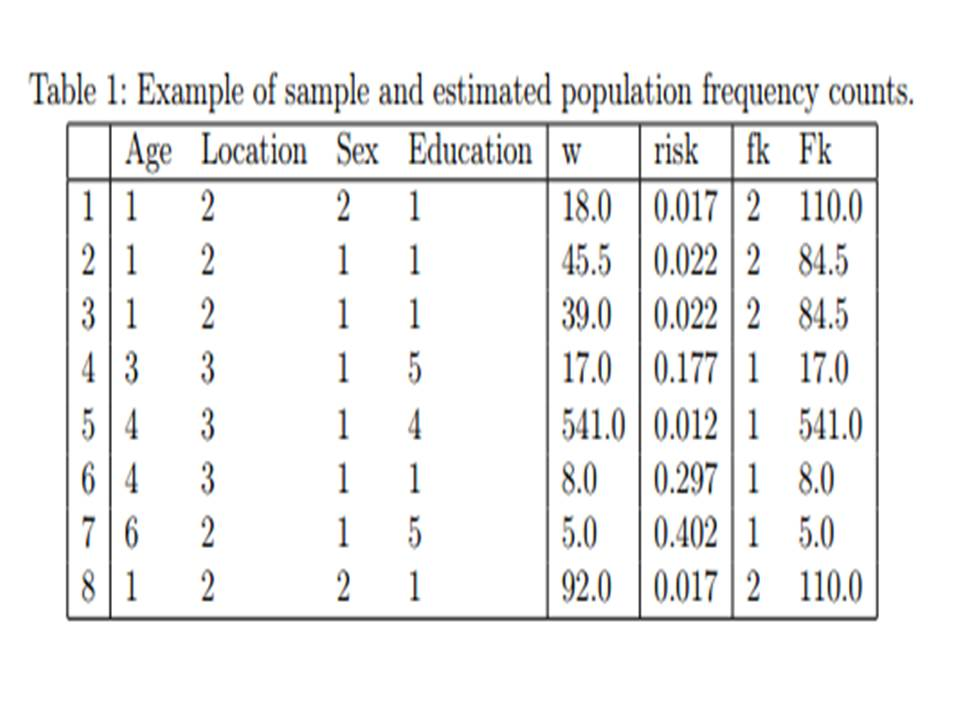
\includegraphics[width=0.9\linewidth]{JPEGS/TemplTable1}
\caption{}
\label{fig:TemplTable1}
\end{figure}

\end{frame}
	%----------------------------------------------------------------------------%
	\begin{frame}	
		\frametitle{Population Frequencies}
		
\begin{itemize}
	\item In Table 1 a very simple data set is used to explain the calulation of sample
	frequency counts and the (first rough) estimation of population frequency counts.
	One can easily see that observation 1 and 8 are equal, given the key-variables Age
	Class , Location, Sex and Education. Because the values of observations 1 and
	8 are equal and therefore the sample frequency counts are $f_1=2$ and $f_8=2$.
\end{itemize}
\end{frame}
%----------------------------------------------------------------------------%
\begin{frame}	
	\frametitle{Population Frequencies}
	
	\begin{itemize}
	\item Estimated population frequencies are obtained by summing up the sample weights
	for equal observations. 
	\item Population frequencies $\hat{F}_1$ and $\hat{F}_8$ can then be estimated
	by summation over the corresponding sampling weights, $w_1$ and $w_8$. 
	\item In summary,
	two observations with the pattern (key) (1,2,5, 1) exist in the sample and 110
	observations with this pattern (key) can be expected to exist in the population.
\end{itemize}
\end{frame}

	%----------------------------------------------------------------------------%
	\begin{frame}	
		\frametitle{Population Frequencies}
		
%----------------------------------------------------------------------------%
% % Graphic
% % Table 1: Example of sample and estimated population frequency counts.
% % TemplTable1.jpg

%----------------------------------------------------------------------------------------%
\end{frame}
	%----------------------------------------------------------------------------%
	\begin{frame}	
		\frametitle{Population Frequencies}
		
		\begin{itemize}
	\item One can show, however, that these estimates almost always overestimate small
	population frequency counts .
	%see, e.g., Templ and l\leill<ll, 2010].
	
	\item A better approach is to use so-called super—population models, in which population frequency
	counts are modeled given certain distributions. 
	
	\item For example, the estimation procedure of sample counts given the population counts can be modeled by assuming
	a negative binomial distribution and is implemented
	in \textbf{sdcMicro} in function \texttt{measurelisk()}
	and called by the
	\textbf{sdcMicroGUI}.
\end{itemize}	
\end{frame}
	%----------------------------------------------------------------------------%
	\begin{frame}	
		\frametitle{Population Frequencies}
		
\begin{figure}
\centering
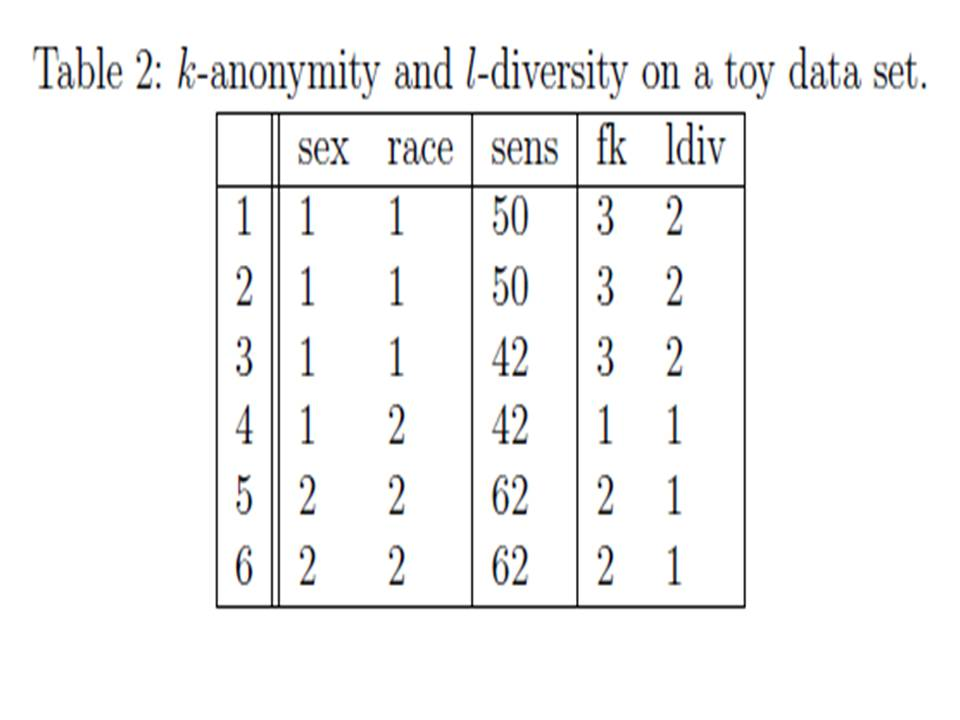
\includegraphics[width=0.99\linewidth]{TemplJPGs2/Table2}
\caption{}
\label{fig:Table2}
\end{figure}

%%Page 7 / 31
%--------------------------------------------------------------------

%2 MEASURING THE DISCLOSURE RISK
%Table 2: is-anonymity and l-diversity on a toy data set.
\end{frame}

\begin{frame}
	\frametitle{k-anonymity}
	\begin{itemize}
		\item \textbf{k-anonymity} is a property possessed by certain anonymized data. 
		\item The concept of k-anonymity was first formulated by Latanya Sweeney in a paper published in 2002 as an attempt to solve the problem: 
		\begin{quote}"Given person-specific field-structured data, produce a release of the data with scientific guarantees that the individuals who are the subjects of the data cannot be re-identified while the data remain practically useful."
		\end{quote}
	\end{itemize}
\end{frame}
\begin{frame}
	\frametitle{k-anonymity}
	\begin{itemize}
		\item A release of data is said to have the k-anonymity property if the information for each person contained in the release cannot be distinguished from at least k-1 individuals whose information also appear in the release. 
		\item The various procedures and programs for generating anonymised data providing k-anonymity protection have been patented in the United States.
	\end{itemize}
\end{frame}

\begin{frame}
\begin{itemize}
	\item l-diversity is a form of group based anonymization that is used to preserve privacy in data sets by reducing the granularity of a data representation.
	\item This reduction is a trade off that results in some loss of effectiveness of data management or mining algorithms in order to gain some privacy. 
	\item The l-diversity model is an extension of the k-anonymity model which reduces the granularity of data representation using techniques including generalization and suppression such that any given record maps onto at least k other records in the data. 
	\end{itemize}
\end{frame}

\begin{frame}
	\begin{itemize}	\item The l-diversity model handles some of the weaknesses in the k-anonymity model where protected identities to the level of k-individuals is not equivalent to protecting the corresponding sensitive values that were generalized or suppressed, especially when the sensitive values within a group exhibit homogeneity. 
	\item The l-diversity model adds the promotion of intra-group diversity for sensitive values in the anonymization mechanism.
\end{itemize}
\end{frame}
	%======================================================%
	\begin{frame}
		\frametitle{Measuring Risk : k-anonymity}
		\begin{itemize}
			\item Based on a set of key variables, one desired characteristic of a protected micro
			dataset is often to achieve \textbf{k-anonymity} 
			%[Samarati and Sweeney, 1998, Sarnarati,2001, Swwriey, 2002]. 
			\item This means that each possible pattern of key variables con-
			tains at least k units in the microdata. This is equal to $f_i \geq k, i=1,2,3,\ldots ,n$.  A
			typical value is k = 3.
			\item k—anonymity is typically achieved by recoding categorical key variables into fewer
			categories and by suppressing specific values of key variables for some units;
		\end{itemize}
		% see Section 3.1 and 3.2.
	\end{frame}
	
	%======================================================%
	\begin{frame}
		\frametitle{Measuring Risk : l-diversity}
		\begin{itemize}	
			\item An extension of k-anonymity is l-diversity. Consider
			a group of observations with the same pattern/keys in the key variables and let
			the group fulfill k-anonymity. \item A data intruder can therefore by definition not
			identify an individual within this group. 
			\item If all observations have the same entries
			in an additional sensitive variable. however (e.g., cancer in the variable medical
			diagnosis), an attack will be successful if the attacker can identify at least one
			individual of the group, as the attacker knows that this individual has cancer
			with certainty. 
			\item The distribution of the target-sensitive variable is referred to as
			l-diversity.
		\end{itemize}
	\end{frame}
	
	\begin{frame}
		\begin{figure}
			\centering
			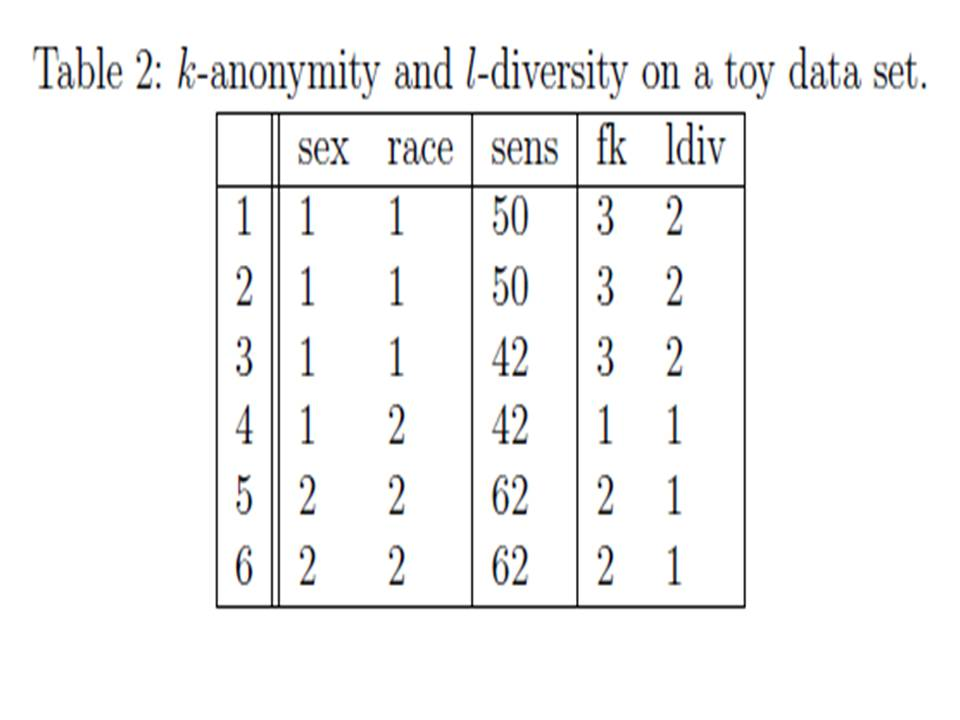
\includegraphics[width=0.7\linewidth]{TemplJPGs2/Table2}
			\caption{}
			\label{fig:Table2}
		\end{figure}
		
	\end{frame}
	%======================================================%
	\begin{frame}
		%======================================================%
		\begin{itemize}
			\item		Table 2 considers a small example dataset that highlights the calculations of
			l-diversity.
			\item  It also points out the slight difference compared to k-anonymity. The
			first two columns present the categorical key variables. 
			\item The third column of the
			data defines a variable containing sensitive information. 
		\end{itemize}
	\end{frame}
	
	%======================================================%
	\begin{frame}	
		\begin{itemize}
			\item Sample frequency counts $f_i$ appear in the fourth column. They equal 3 for the first three observations; the
			fourth observation is unique and frequency counts $f_i$ are 2 for the last two observations. 
			\item Only the fourth observation violates 2-anonymity. Looking closer at the first
			three observations, we see that only two different values are present in the sensitive
			variable. 
			\item Thus the l-(distinct) diversity is just 2. 
		\end{itemize}
		%----------------------------------------------------------------------------%
	\end{frame}
	%======================================================%
	\begin{frame}
		\begin{itemize}
			\item For the last two observations,
			2-anonymity is achieved, but the intruder still knows the exact information of the
			sensitive variable. \item For these observations, the l-diversity measure is 1. indicating
			that sensitive information can be disclosed, since the value of the sensitive variable
			is = 62 for both of these observations.
		\end{itemize}
	\end{frame}
	%======================================================%
	\begin{frame}
		\begin{itemize}
			\item Diversity in values of sensitive variables can be measured differently. We present
			here the distinct diversity that counts how many different values exist within a
			pattern. 
			\item Additional methods such as entropy, recursive and multi-recursive are implemented in \textbf{sdcMicro}.
		\end{itemize}
	\end{frame}
	
	%======================================================%
	\begin{frame}
		
		%======================================================%
		\frametitle{Special Uniques Detection Algorithm (SUDA)}
		\begin{itemize}
			\item The \textbf{Special Uniques Detection Algorithm (SUDA)} is an often discussed method
			to estimate the risk, but applications of this method can be rarely found. 
			\item For
			the sake of completeness this algorithm is implemented in sdcMicro (but not in
			sdcMicroGUI) and explained in this document, but to evaluate the usefulness of
			this method it needs more research. 
			
			\item In the following the interested reader will
			see that the SUDA approach is more than the sample frequency estimation shown
			before. 
			\item It consider also subsets of key variables. SUDA estimates disclosure risks
			for each unit. SUDA2  is the computationally improved
			version of SUDA. 
		\end{itemize}
		%% Cite:  [e.g., Manning et al., 2008]
	\end{frame}
	%======================================================%
	
	\begin{frame}
		\frametitle{SUDA2}
		It is a recursive algorithm to find \textbf{\textit{Minimal Sample Uniques}}
		(MSUs). SUDA2 generates all possible variable subsets of selected categorical key
		variables and scans for unique patterns within subsets of these variables. The risk
		of an observation primarily depends on two aspects:
		%---------------------------------------------------------------------------------------%
		
		\begin{itemize}
			\item[(a)] The lower the number of variables needed to receive uniqueness, the higher
			the risk (and the higher the SUDA score) of the corresponding observation.
			\item[(b)] The larger the number of minimal sample uniqueness contained within an
			observation, the higher the risk of this observation.
		\end{itemize}
		%---------------------------------------------------------------------------------------%
		
		%_ m—l
		%Item (a) is considered by calculating for each observation 1' by Z, — 1_[k_MSUm,-,,,1(m—
		%la) ,i * I, ..., 11.
	\end{frame}
	
	%======================================================%
	\begin{frame}
		
		In this formula, m corresponds to the depth, which is the max-
		imum size of variable subsets of the key variables, \textit{MSUmin}$_i$, is the number of
		MSUs of observation and i and n are the number of observations of the dataset.
		%---------------------------------------------------------------------------------------%
		\begin{itemize}
			\item Since each observation is treated independently, a specific value 1,; belonging to a
			specific pattern are summed up. This results in a common SUDA score for each
			of the observations contained in this pattern; this summation is the contribution
			mentioned in item 
			\item The final SUDA score is calculated by normalizing these SUDA scores by dividing them by pl, with p being the number of key variables.
		\end{itemize}
	\end{frame}
	%======================================================%
	\begin{frame}
		\frametitle{Data Intrusion Score}
		\begin{itemize} 
			\item To receive the so-called
			\textbf{Data Intrusion Simulation (DIS) score}, loosely speaking, an iterative algorithm
			based on sampling of the data and matching of subsets of the sampled data with
			the original data is applied. 
			\item This algorithm calculates the probabilities of correct
			matches given unique matches. It is, however, out of scope to precisely describe
			this algorithm here. %reference Fllliot [2000] for details. 
		\end{itemize}
	\end{frame}
	%======================================================%
	\begin{frame}
		\frametitle{Data Intrusion Score}
		\begin{itemize} 
			\item The DIS SUDA score is calculated from the SUDA and DIS scores, and is available in \textbf{sdcMicro} as \texttt{disScore()}.
			\item Note that this method does not consider population frequencies in general, but
			does consider sample frequencies on subsets. 
			\item The DIS SUDA scores approximate
			uniqueness by simulation based on the sample information population, but to our
			knowledge, they generally do not consider sampling weights, and biased estimates
			may therefore result.
		\end{itemize}
	\end{frame}
	%======================================================%
	\begin{frame}
		\frametitle{Data Intrusion Score}
		\begin{itemize} 			
			%	\item In Table 3, we use the same test dataset as in Section 2.1. 
			\item Sample frequency
			counts $f_i$ as well as the SUDA and DIS SUDA scores have been calculated. 
			\item The
			SUDA scores have the largest value for observation 4 and 6 since subsets of key
			variables of these observation are also unique, while for observations 1 — 3, 5 and
			8, less subsets are unique.
		\end{itemize}
	\end{frame}
	
	%======================================================%
	\begin{frame}
		%%--- Page 9 / 31
		%--------------------------------------------------------------------------------------------------------%
		% 2 MEASURING THE DISCLOSURE RISK
		Table 3: Example of SUDA scores (scores) and DIS SUDA scores (disScores).
		\begin{figure}
			\centering
			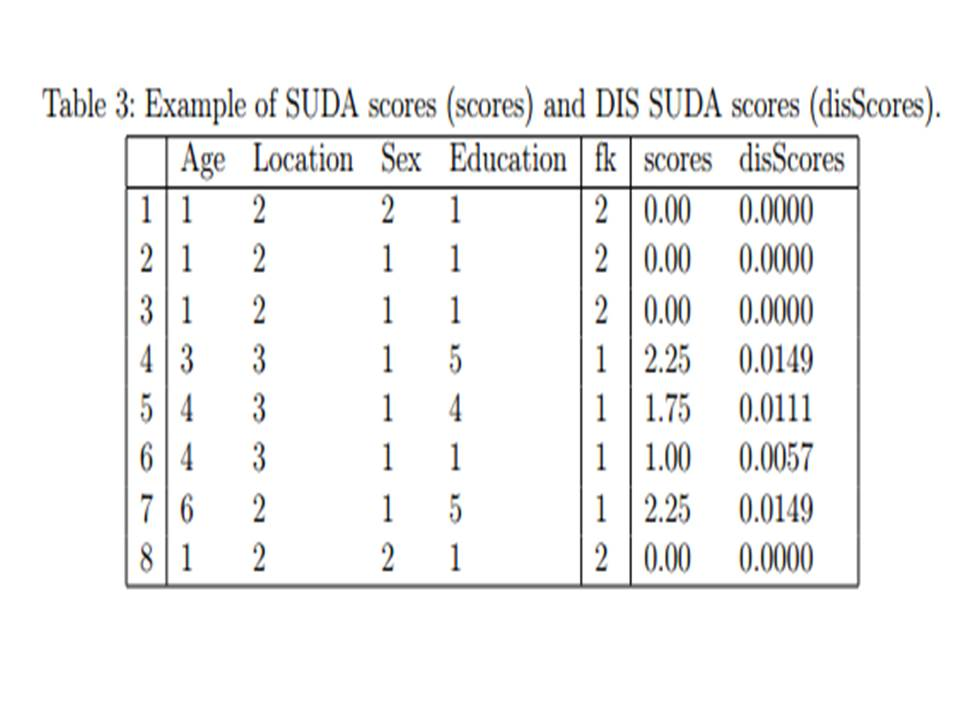
\includegraphics[width=0.99\linewidth]{JPEGS/TemplTable3}
			\caption{}
			\label{fig:TemplTable3}
		\end{figure}
		
		%%% TemplTable3.jpg
	\end{frame}
	%======================================================%
	\begin{frame}
		%----------------------------------------------------------------------------------------------%
		In sdcMicro (function \texttt{suda2()}) additional output, such as the contribution
		percentages of each variable to the score, are available. The contribution to the
		SUDA score is calculated by assessing how often a category of a key variable
		contributes to the score.
	\end{frame}
	%======================================================%
	\begin{frame}
		\frametitle{Calculating Cluster (Household) Risks}
		\begin{itemize}
			\item Micro datasets often contain hierarchical cluster structures; an example is social
			surveys, when individuals are clustered in households. 
			\item The risk of re-identifying
			an individual within a household may also affect the probability of disclosure of
			other members in the same household. Thus, the household or cluster-structure of
			the data must be taken into account when calculating risks.
		\end{itemize}
	\end{frame}
	%======================================================%
	\begin{frame}
		\frametitle{Calculating Cluster (Household) Risks}
		\begin{itemize}			
			\item It is commonly assumed that the risk of re-identfication of a household is the risk
			that at least one member of the household can be disclosed. Thus this probability
			can be simply estimated from individual risks as 1 minus the probability that no
			member of the household can be identfied. 
			\item Thus, if we consider a single household
			with three persons that have individual risks of re-identification of 0.1, 0.05 and
			0.01, respectively, the risk-measure for the entire household will be calculated as
			1-(0.1+0.05+0.01). 
			\item This is also the implementation strategy from \textbf{sdcMicro}.
		\end{itemize}
	\end{frame}
\end{document}
		